\begin{itemize}
    \item Consider clustering over graph data, that is, given a graph, the goal is to cluster the nodes by using the edges and their weights, which represent the similarity between the incident nodes.
    \item Similarity is a relative quantity between two instances, High when similar and Low when dissimilar.\textbf{Distance is a dissimilarity measure.}
    \item For n data instances,We have ($n^2$) similarities to be computed and pack them into a similarity matrix (A) where it can be viewed as weighted adjacency matrix of a graph.
    \begin{figure}[H]
        \centerline{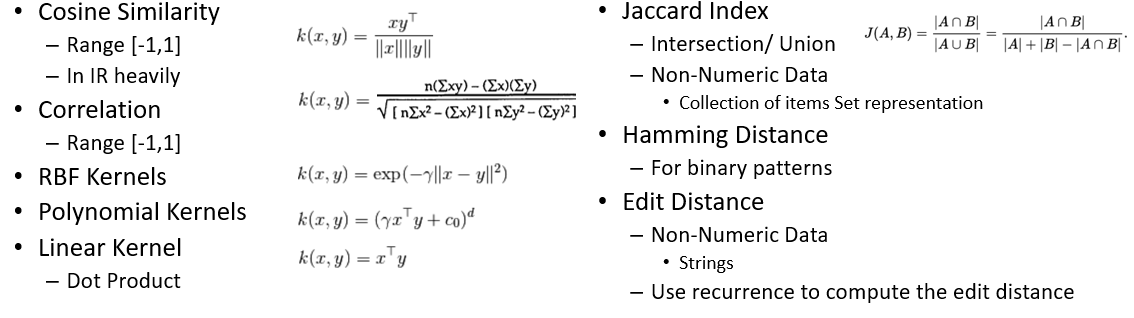
\includegraphics[width=1.5\textwidth]{Figures/sim.png}}
        \caption{\label{fig:figure5}Similarity Measures}
    \end{figure}
    \item In graph theory, a minimum cut of a graph is a cut that partition graph into two sets A and B such that weight of edges connecting vertices in A to vertices in B is minimum.
    \item Easy to solve O(VE) algorithm But Not satisfactory partition as it tends often to isolate vertices
    \begin{figure}[H]
        \centerline{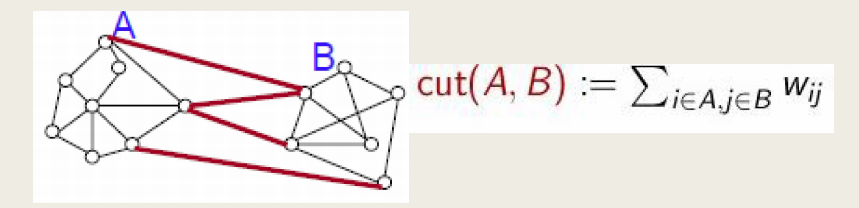
\includegraphics[width=\textwidth]{Figures/mincut.png}}
        \caption{\label{fig:figure6}Minimum Cut Rule}
    \end{figure}
    \item Normalized cut however works to partition graph into two sets A and B such that weight of edges connecting vertices in A to vertices in B is minimum and size of A and B are very similar.
    \item However, the main problem we face is that the eigenvectors u i are not binary, and thus
    it is not immediately clear how we can assign points to clusters. One solution to this
    problem is to treat the n x k matrix of eigenvectors as a new data matrix.
    \begin{figure}[H]
        \centerline{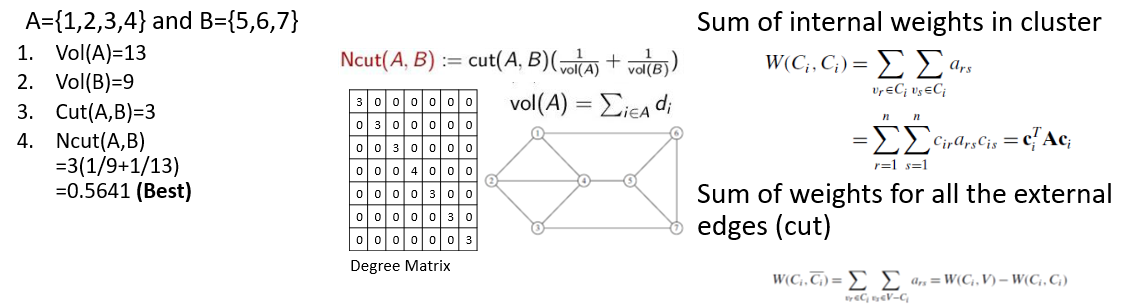
\includegraphics[width=1.6\textwidth]{Figures/normcut.png}}
        \caption{\label{fig:figure7}Normalized Cut}
    \end{figure}
    \begin{figure}[H]
        \centerline{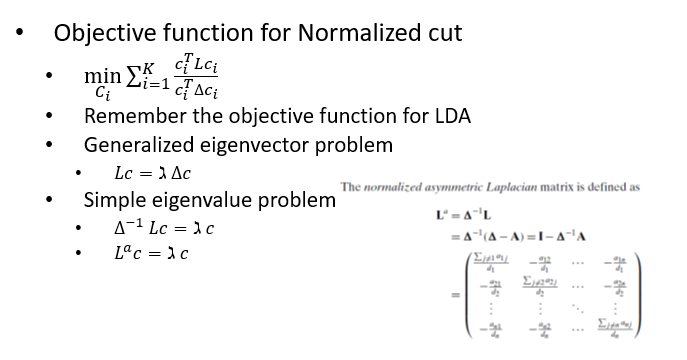
\includegraphics[width=1.4\textwidth]{Figures/spectral2.png}}
        \caption{\label{fig:figure8}Spectral Clustering Objective Function}
    \end{figure}
    \begin{figure}[H]
        \centerline{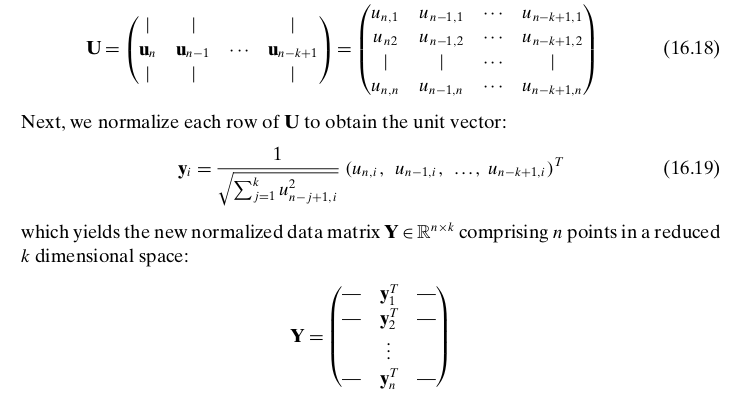
\includegraphics[width=1.2\textwidth]{Figures/yspectral.png}}
        \caption{\label{fig:figure9}Normalized Eigenvectors}
    \end{figure}
    \item \textbf{Applying k-means to Laplacian eigenvectors allows us to find cluster with non-convex boundaries.}
    \item Some Issues are the choice of number of clusters k, choice of similarity measure, for RBF Gaussian kernels, choice of $\gamma$.
    \item Complexity is as follows, Construction of the similarity matrix O($n^2$d)and Eigenvalue decomposition O($n^3$)
    \begin{figure}[H]
        \centerline{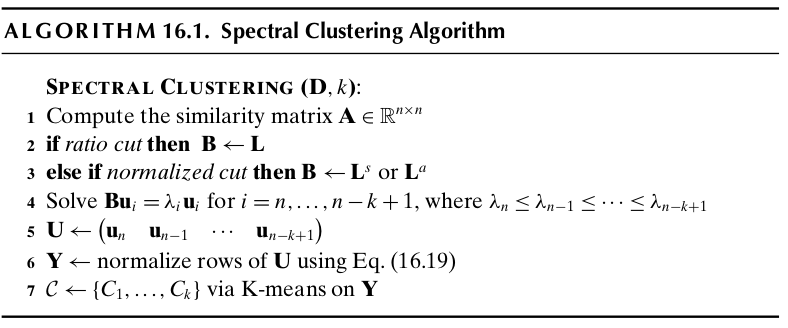
\includegraphics[width=\textwidth]{Figures/spectral.png}}
        \caption{\label{fig:figure10}Normalized Cut Algorithm}
    \end{figure}
\end{itemize}